\documentclass[11pt]{article}
\usepackage[a4paper,margin=24mm]{geometry}
\usepackage{graphicx,booktabs,amsmath}
\begin{document}
\section*{Matched-protocol $\alpha$-Ti phonons: DFT-PBEsol and DPA4}
The DPA4-finetuned-PBEsol checkpoint 23100 was evaluated on the exact three
DFT POSCAR files: the undisplaced reference and the two opposite
$0.01$~\AA\ displacements. No relaxation was performed. The cell contained
96 atoms ($4\times4\times3$). Slurm job 20972853 completed on CPU node
apollo26 in 35 seconds; output checksums were verified after collection.

Both force sets were processed by the same Phonopy functions: subtract
reference forces, remove mean force, retain the antisymmetric central pair,
fit full force constants, apply the symfc projector and ten numerical
translation/permutation polishing cycles. The mass is 47.867 amu.
The DOS uses a Gamma-centred $50^3$ mesh and Gaussian $\sigma=0.05$ THz;
both integrals are 3 modes per atom. Previous DFT force constants are
reproduced exactly. Neither spectrum has modes below $-0.001$ THz on
the mesh or the plotted path.

\begin{center}
\begin{tabular}{lrr}\toprule
Quantity & DFT-PBEsol & DPA4 \\\midrule
Upper optical frequency at Gamma (THz) & 5.7575 & 4.9542 \\
Main DOS peak in 7--7.6 THz (THz) & 7.194 & 7.328 \\
Peak height (modes/atom/THz) & 0.7815 & 1.0068 \\
Low-frequency DOS peak (THz) & 3.252 & 3.510 \\\bottomrule
\end{tabular}
\end{center}
The discrepancy in the optical peaks persists under the matched protocol.
It therefore cannot be explained solely by the different geometries,
supercells, or force-processing methods used in the preceding comparison.
This is a comparison at the current DFT settings (550 eV, electronic
$6^3$ mesh, electronic Gaussian smearing 0.1 eV); convergence in these
parameters and supercell size remains unestablished. The sorted-frequency
path RMSE is 0.276 THz, without eigenvector-based branch tracking.
The central-force component RMSE is $2.825\times10^{-4}$ eV/\AA.

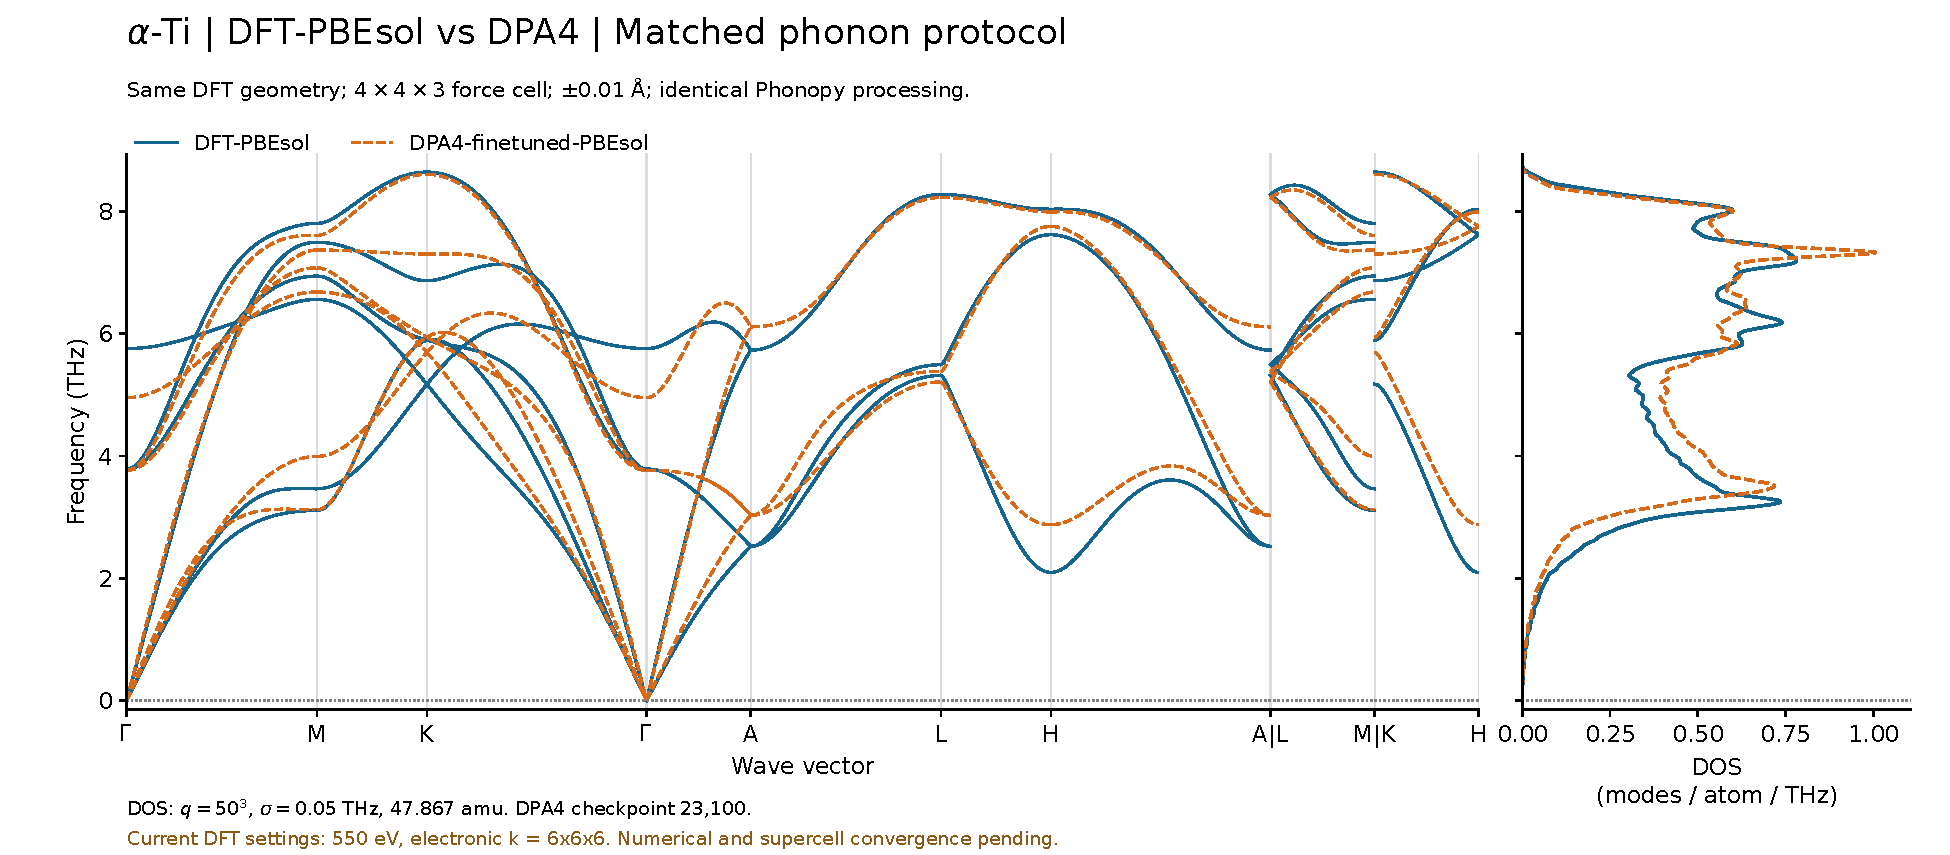
\includegraphics[width=\textwidth]{matched-bands-DOS.pdf}
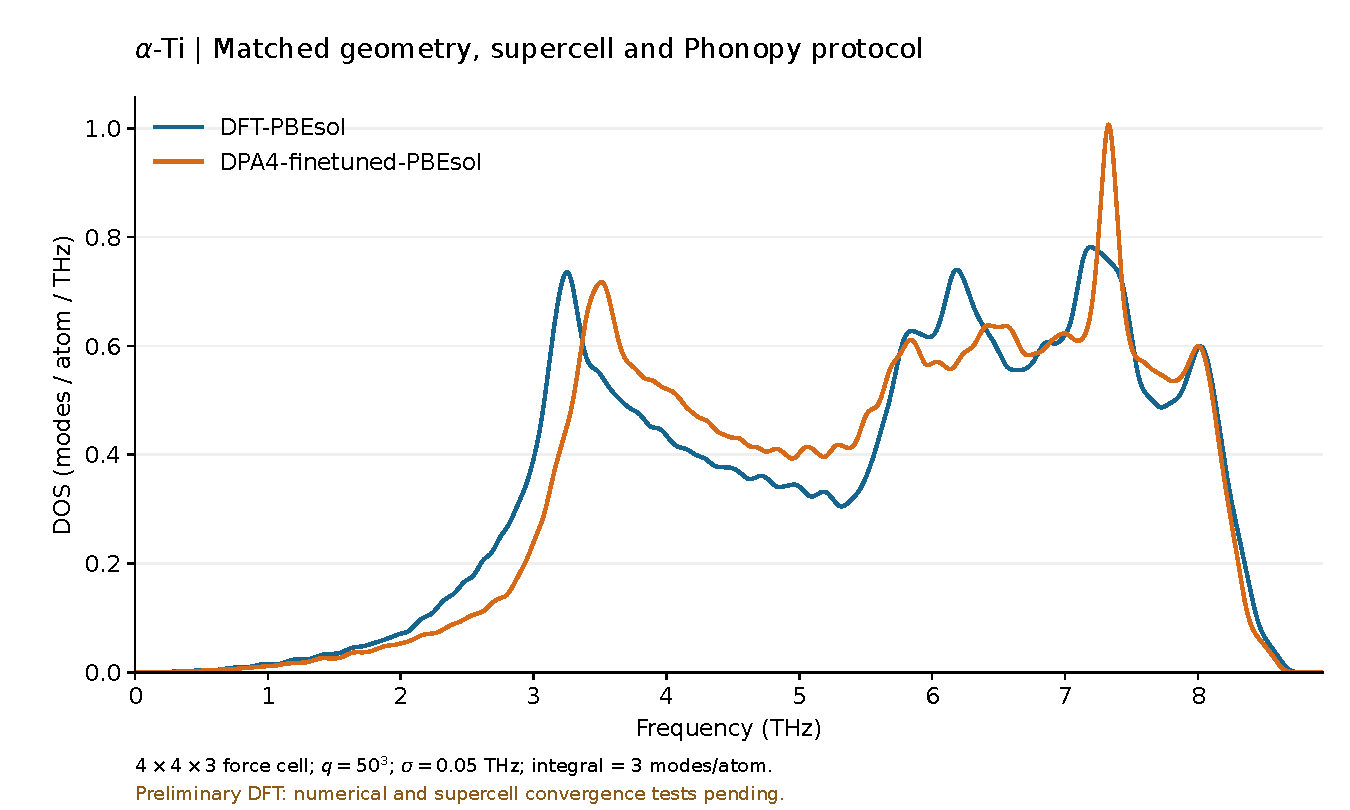
\includegraphics[width=\textwidth]{matched-DOS.pdf}
\end{document}
